\documentclass [11pt ,a4paper ,twoside ]{article}
\title{\textbf{Spider-chase}}
\author{Marco Mecchia\\
		Luigi Giugliano\\
		Simone Romano}
\date{}

\usepackage{mathtools}
\usepackage{listings}
\usepackage[italian]{babel}
\usepackage{color}
\usepackage{graphicx}
\usepackage{hyperref}


\definecolor{mygreen}{rgb}{0,0.6,0}
\definecolor{mygray}{rgb}{0.5,0.5,0.5}
\definecolor{mymauve}{rgb}{0.58,0,0.82}

\lstdefinestyle{c}{ %
  backgroundcolor=\color{white},   
  basicstyle=\footnotesize,
  breakatwhitespace=false, 
  breaklines=true,               
  captionpos=b,                    
  commentstyle=\color{mygreen},    
  deletekeywords={...},
  escapeinside={\%*}{*)},
  extendedchars=true,
  frame=single,
  keepspaces=true,
  keywordstyle=\color{blue},
  language=C,
  otherkeywords={*,...},
  numbers=left,
  numbersep=5pt,
  numberstyle=\tiny\color{mygray},
  rulecolor=\color{black},
  showspaces=false,
  showstringspaces=false,
  showtabs=false,
  stepnumber=1,
  stringstyle=\color{mymauve},     
  tabsize=2,	                   
  title=\lstname
}

\lstdefinestyle{python}{ %
  backgroundcolor=\color{white},   
  basicstyle=\footnotesize,
  breakatwhitespace=false, 
  breaklines=true,               
  captionpos=b,                    
  commentstyle=\color{mygreen},    
  deletekeywords={...},
  escapeinside={\%*}{*)},
  extendedchars=true,
  frame=single,
  keepspaces=true,
  keywordstyle=\color{blue},
  language=Python,
  otherkeywords={*,...},
  numbers=left,
  numbersep=5pt,
  numberstyle=\tiny\color{mygray},
  rulecolor=\color{black},
  showspaces=false,
  showstringspaces=false,
  showtabs=false,
  stepnumber=1,
  stringstyle=\color{mymauve},     
  tabsize=2,	                   
  title=\lstname
}

\lstdefinestyle{javascript}{ %
  backgroundcolor=\color{white},   
  basicstyle=\footnotesize,
  breakatwhitespace=false, 
  breaklines=true,               
  captionpos=b,                    
  commentstyle=\color{mygreen},    
  deletekeywords={...},
  escapeinside={\%*}{*)},
  extendedchars=true,
  frame=single,
  keepspaces=true,
  keywordstyle=\color{blue},
  language=Javascript,
  otherkeywords={*,...},
  numbers=left,
  numbersep=5pt,
  numberstyle=\tiny\color{mygray},
  rulecolor=\color{black},
  showspaces=false,
  showstringspaces=false,
  showtabs=false,
  stepnumber=1,
  stringstyle=\color{mymauve},     
  tabsize=2,	                   
  title=\lstname
}

\begin{document}
\maketitle

\tableofcontents

\cleardoublepage

\section{Introduzione}

Lo scopo del progetto "Spider-chase" \'e quello di mettere a frutto le conoscenze acquisite nel corso di robotica, sperimentando varie soluzioni riguardanti robot mobili. In particolare, nel nostro progetto abbiamo deciso di utilizzare dei ragni robot DIY (Do It Yourself) dal basso costo, controllati dal microcontrollore STM32 Nucleo. Questa scelta ci ha consentito di:

\begin{itemize}
\item Sperimentare con componenti economici.
\item Montare i robot in maniera autonoma, senza fare affidamento su prodotti precostruiti, in modo da poter fare modifiche strutturali anche in corso d'opera.
\item Utilizzare ChiBiOs, un sistema operativo embedded fornito da STM, in modo da poter programmare i robot in maniera astratta ed evitare la programmazione \textit{bare metal}.
\end{itemize}

\subsection{Requisiti funzionali}
Ad inizio progetto ci siamo proposti i seguenti requisiti funzionali:
\begin{itemize}
\item Ogni ragno deve essere in grado di muoversi liberamente nello spazio, in qualunque direzione.
\item Ogni ragno deve essere in grado di ricevere istruzioni via wireless.
\item Ogni ragno deve essere alimentato in maniera autonoma e non deve essere vincolato a sorgenti di alimentazione fisse.
\item Un ragno deve essere in grado di stabilire la posizione di un altro ragno ed eventualmente inseguirlo.
\end{itemize}

Tali requisiti sono stati tutti soddisfatti dal risultato finale.

\section{Architettura e componenti}

Nel progetto abbiamo utilizzato i seguenti componenti:
\begin{itemize}
\item 6 ragni meccanici DIY, ciascuno con un motore.
\item 3 schede STM Nucleo.
\item 3 moduli wireless (modello).
\item 3 driver per motori (modello).
\item 1 webcam.
\item 1 pc.
\item 1 controller Xbox.
\item 1 cellulare Android.
\end{itemize}

L'architettura totale pianificata \'e mostrata in figura. 

\begin{center}
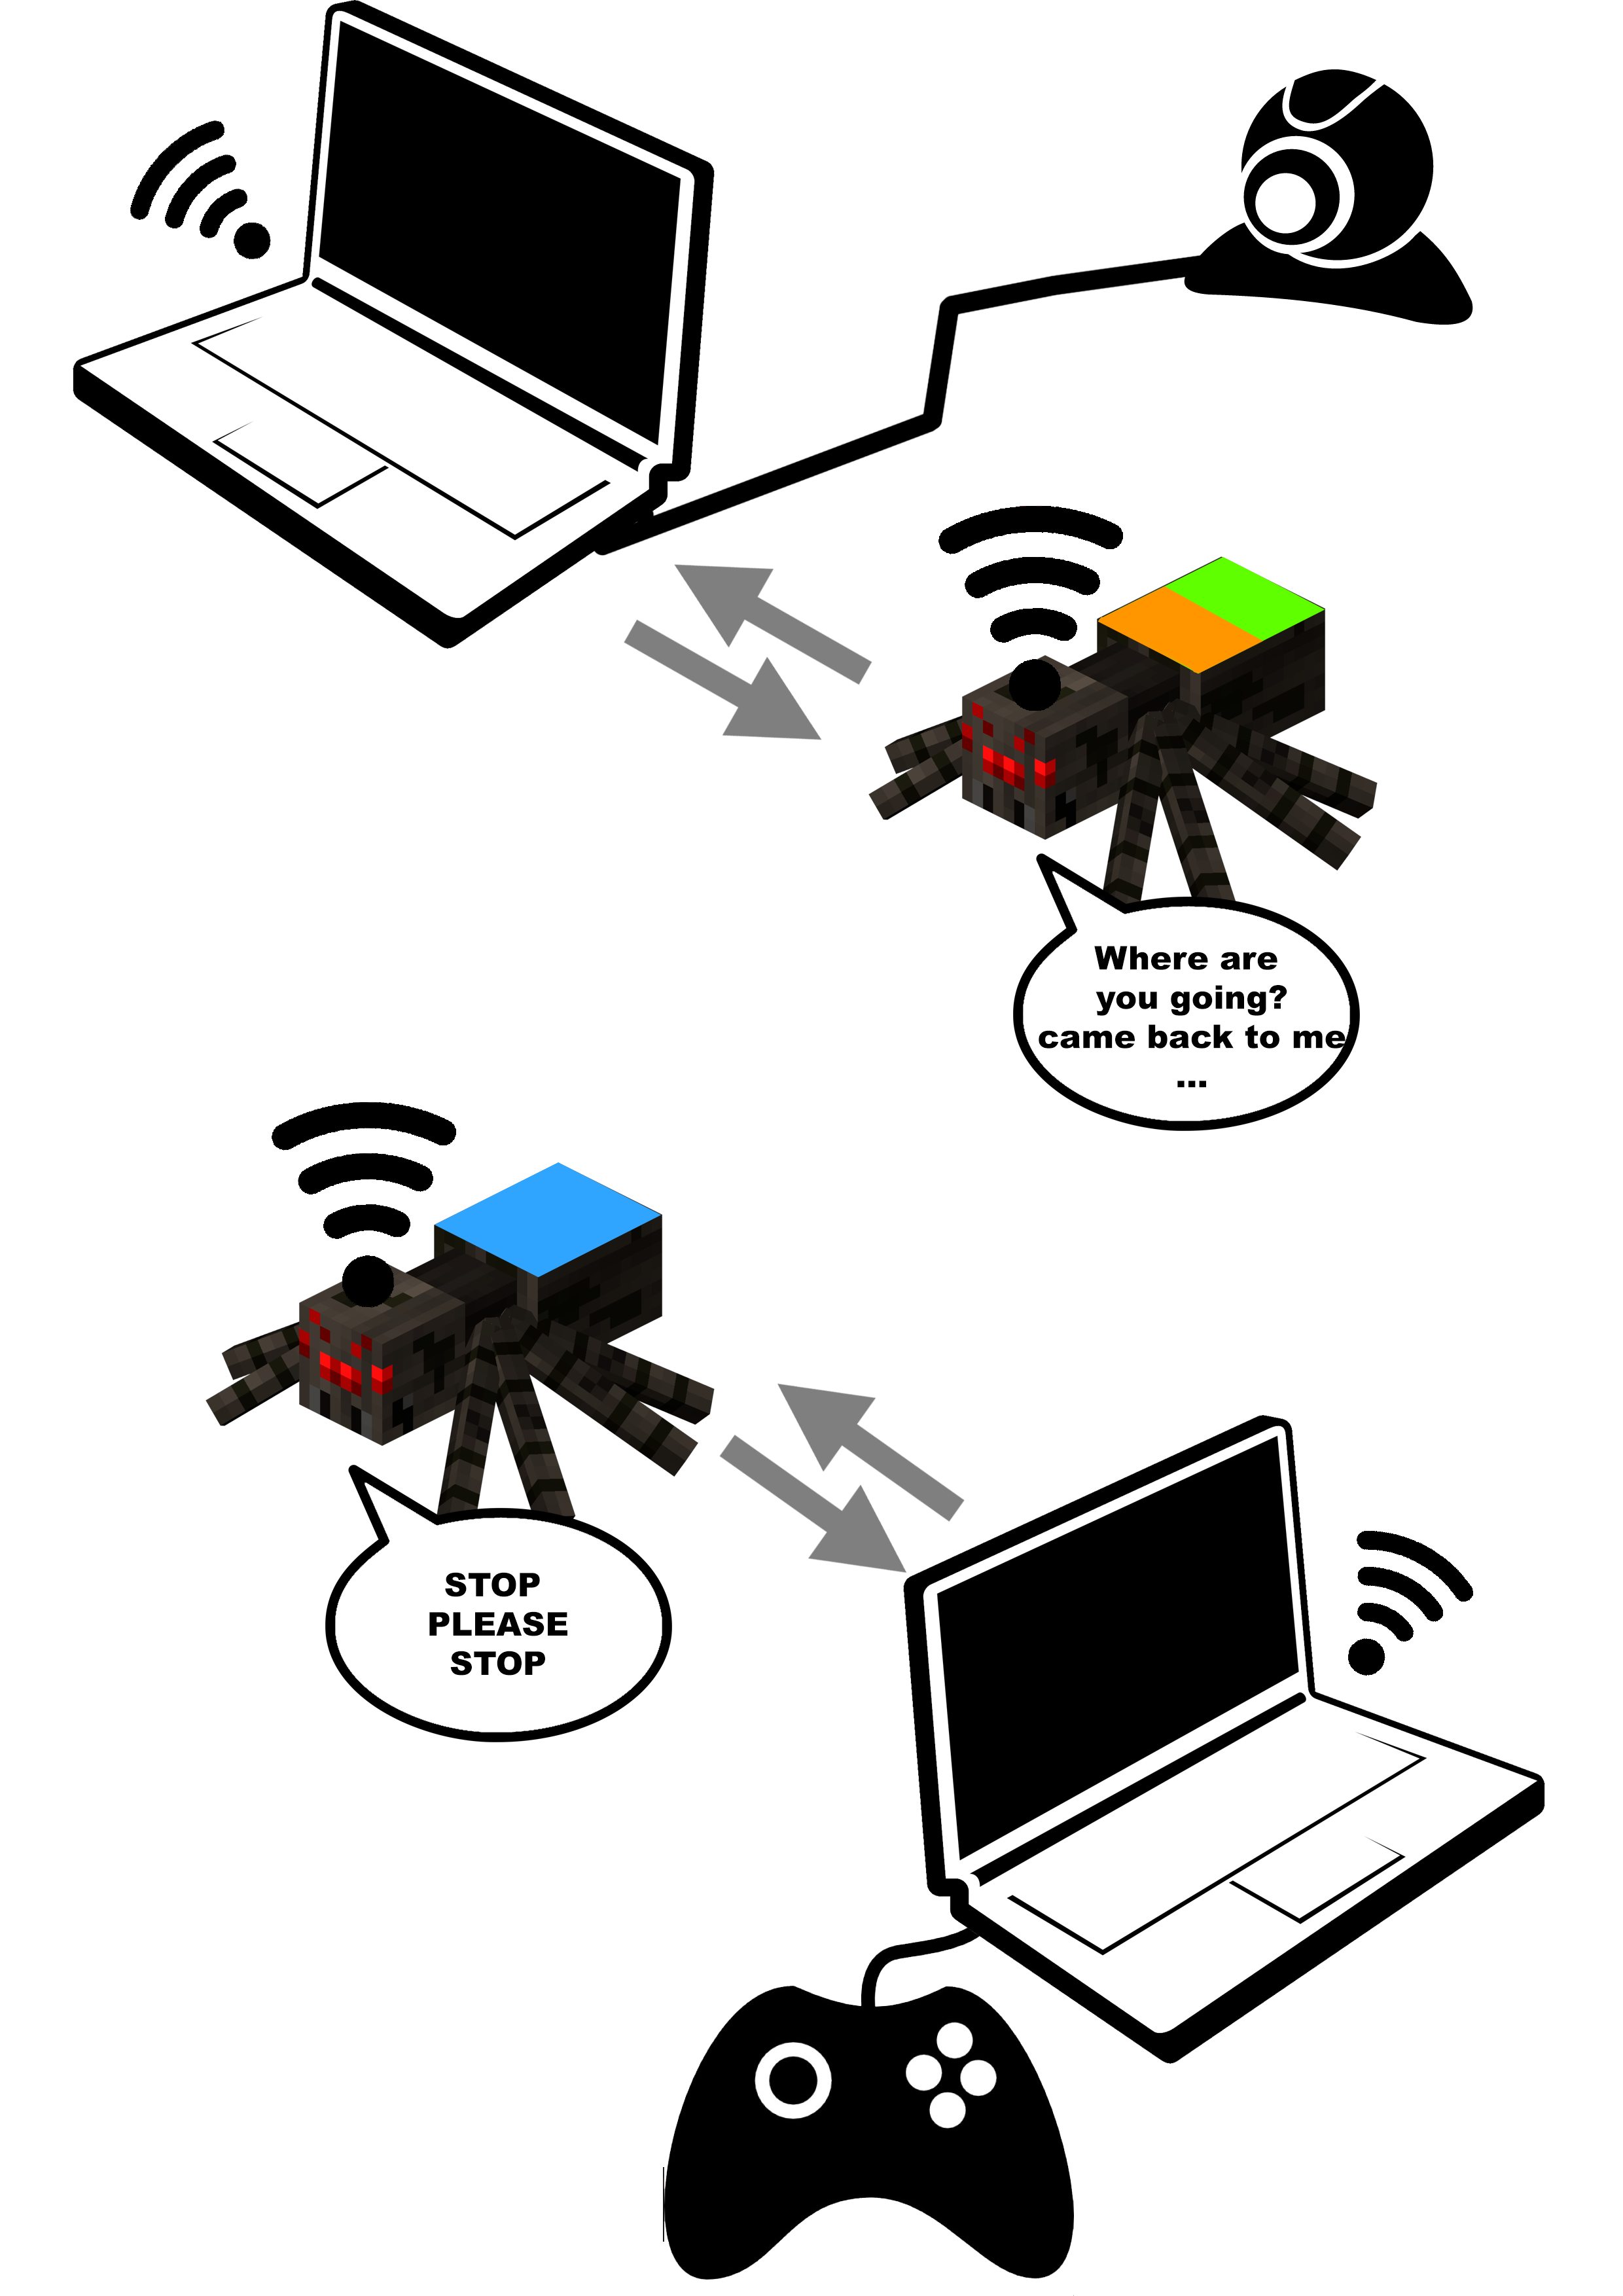
\includegraphics[keepaspectratio, width=200pt]{Images/Infographic.png}
\end{center}

Tutti e tre i ragni possono ricevere messaggi wireless che impostano le velocit\'a dei motori. Ricevuto il messaggio, la board regola le velocit\'a tramite il driver. Il requisito di localizzazione \'e soddisfatto da un modulo di visione artificiale: una webcam posta in alto riconosce i ragni, ed il pc alla quale \'e collegata invia messaggi direttamente ai ragni tramite WiFi. Inoltre, \'e possibile comandare i ragni tramite un cellulare Android od un pc, selezionando il ragno al quale si vogliono impartire i comandi. Ogni ragno \'e alimentato in maniera indipendente da 4 pile stilo poste in un portapile al di sotto del ragno stesso.

\subsection{Ragni meccanici}

I ragni meccanici che abbiamo comprato, mostrati in figura, utilizzano un solo motore per muovere sia le zampe a sinistra che quelle a destra. 
\begin{center}
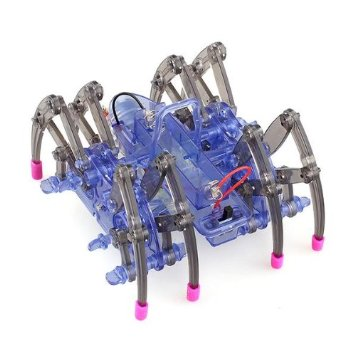
\includegraphics[keepaspectratio, width=300pt]{Images/single_spider2.png}
\end{center}
Bench\'e questa semplice soluzione sia sufficiente a far muovere il ragno avanti e indietro a velocit\'a prefisse, essa non andava incontro al nostro requisito di potersi muovere in qualsiasi direzione dello spazio. Per questo motivo, abbiamo rimosso le zampe a destra di tre ragni, e quelle di sinistra agli altri tre. Unendo i ragni cos\'i divisi, abbiamo ottenuto tre ragni totali, con il pregio di avere motori separati per zampa.
\begin{center}
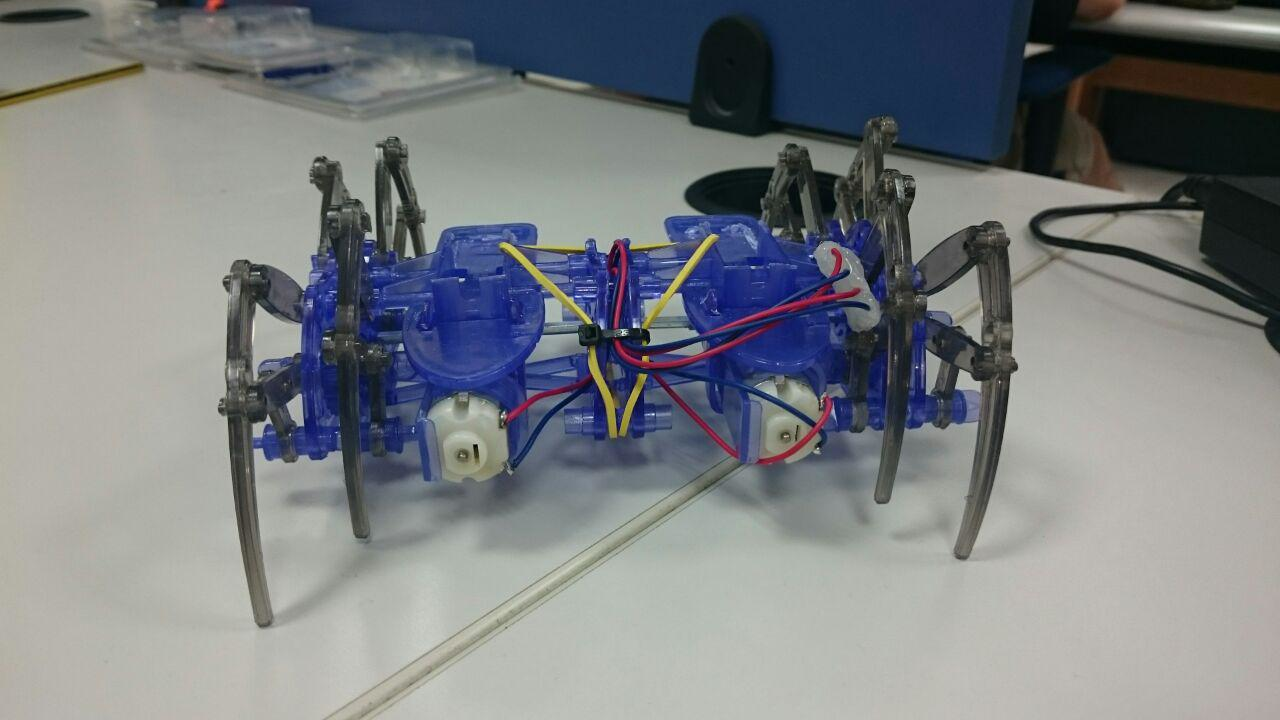
\includegraphics[keepaspectratio, width=300pt]{Images/double_spider.png}
\end{center}
\subsection{STM32F401RE Nucleo}
La board Nucleo STM32 fornisce un'infrastruttura affidabile e flessibile per gli utenti che vogliono sperimentare nuove idee e prototipi che funzionino con tutte la linea di microcontrollori STM32. Grazie al supporto per la connettivit\'a Arduino e ST Morpho, \'e possibile espandere le funzionalit\'a del microcontrollore scegliendo da una vasta gamma di shield. Inoltre, la STM32 nucleo non richiede due ingressi separati per alimentazione e debugging.
\begin{center}
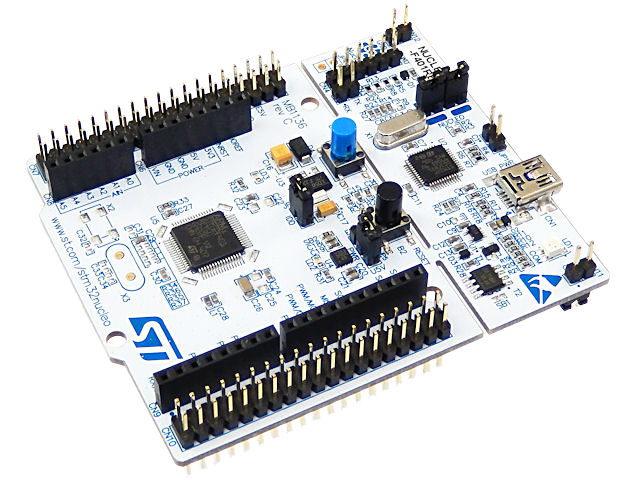
\includegraphics[keepaspectratio, width=200pt]{Images/STM32.png}
\end{center}
\subsection{Driver motore}
Il driver del motore utilizzato \'e il modello L9110s mostrato in figura. 
\begin{center}
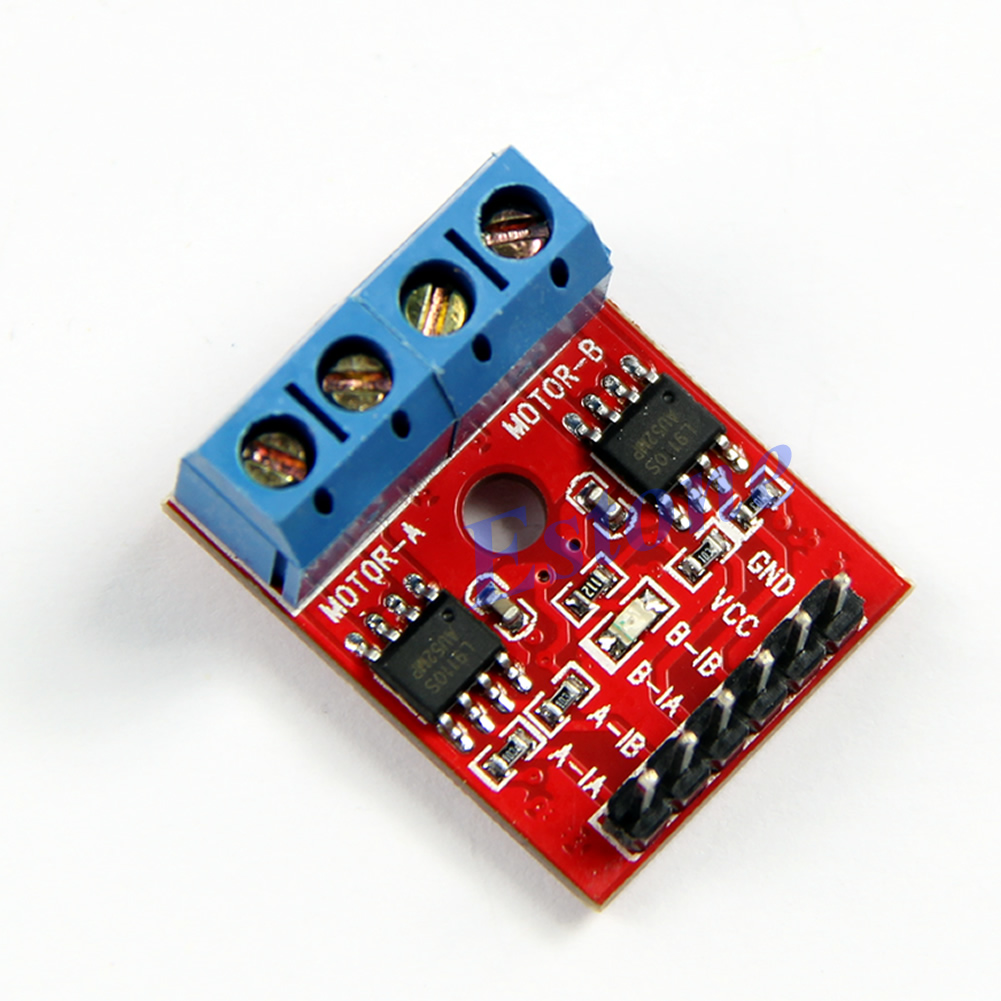
\includegraphics[keepaspectratio, width=200pt]{Images/motor_driver.png}
\end{center}
Dei suoi 10 pin totali, 4 sono di input e 4 di output, 1 di alimentazione e 1 di massa. Quelli in entrata vanno collegati agli output digitali della board, mentre di quelli in uscita 2 sono per il motore destro e 2 per quello sinistro, di cui 1 va all'alimentazione del motore ed uno alla massa. La regolazione della velocit\'a del motore \'e molto semplice e si basa sui PWM che sono collegati agli output digitali della board: se la frequenza del PWM  che arriva all'ingresso 1 \'e maggiore di quella che arriva all'ingresso 2, allora il ragno va in avanti, altrimenti va all'indietro. Maggiore \'e la differenza di, pi\'u il ragno va velocemente.

\subsection{Modulo wireless}
Il modulo wireless utilizzato \'e il modello  mostrato in figura. 
\begin{center}
gayyyy
\end{center}
I suoi pin si collegano, oltre che all'alimentazione ed alla massa, agli ingressi seriali della board. La comunicazione seriale ci ha consentito di comunicare in maniera molto semplice con il modulo, grazie anche agli esempi forniti dalle funzioni di base di ChiBiOs. Il modulo lavora principalmente nello strato di rete, in quanto pu\'o funzionare sia come client che come access point. Inoltre, se impostato come access point, lavora anche nello strato delle applicazioni, in quanto riconosce richieste HTTP di tipo sia GET che POST. Nel nostro caso, abbiamo fatto creare al modulo una rete WiFi, e per mandare messaggi al ragno \'e sufficiente mandare richieste GET tramite browser oppure curl una volta connessi alla rete creata dal modulo.

\subsection{Visione Artificiale e logiche di inseguimento}
Per il modulo di visione artificiale, abbiamo utilizzato lo standard \textit{de facto} nel campo, \textbf{opencv}. Il modulo \'e stato progettato per essere utilizzato con una webcam o una fonte video piazzata in alto rispetto ai ragni. In questo modo, \'e stata semplificata notevolmente la logica di inseguimento, in quanto dal punto di vista del modulo i ragni si muovono su una griglia bidimensionale. Esso riconosce i ragni tramite cartoncini colorati che sono stati messi al di sopra di loro. Una volta riconosciuti entrambi i ragni, il modulo invia un messaggio al ragno inseguitore tramite una richiesta HTTP GET. La logica di inseguimento seguita dal modulo e' molto semplice: Il ragno inseguitore aggiusta il proprio orientamento, cio\'e ruota su se stesso, fin quando gli "occhi" non puntano il ragno inseguito, dopodiche' il ragno prosegue dritto.

\section{Dettagli implementativi}

\subsection{Controller}

\subsection{Driver motore}

Il driver del motore contiene la funzione di inizializzazione, la funzione di controllo del motore date le velocit\'a, ed una funzione di utilit\'a che estrae le due velocit\'a a partire da una stringa.

\lstinputlisting[caption=Motor Driver, style=c]{../RoboWars/MotorController.h}

\subsection{Modulo wireless}

\lstinputlisting[caption=Wireless Module, style=c]{../RoboWars/ESP8266.h}

\subsection{Visione Artificiale}

\lstinputlisting[caption=Vision, style=python]{../Vision/Vision.py}

\section{Conclusioni}

\subsection{Sviluppi futuri}
Il progetto sviluppato ha soddisfatto appieno i requisiti funzionali che ci siamo preposti. Tuttavia, alcuni aspetti potranno essere sicuramente migliorati in futuro:
\begin{itemize}
\item I cartoncini colorati potranno essere sostituiti da markers per la realt\'a aumentata. Ci\'o migliorer\'a il riconoscimento dei ragni ed eliminer\'a la necessit\'a del doppio colore per stabilire l'orientamento del ragno inseguitore. 
\item L'algoritmo di inseguimento potr\'a essere migliorato pianificando traiettorie di curvatura e aggiungendo a bordo del ragno un sensore di prossimit\'a.
\item Si potrebbe eliminare la necessit\'a di un sistema di orientamento globale montando una webcam direttamente sui ragni.
\end{itemize}

\end{document}